%% bare_conf.tex
%% V1.3
%% 2007/01/11
%% by Michael Shell
%% See:
%% http://www.michaelshell.org/
%% for current contact information.
%%
%% This is a skeleton file demonstrating the use of IEEEtran.cls
%% (requires IEEEtran.cls version 1.7 or later) with an IEEE conference paper.
%%
%% Support sites:
%% http://www.michaelshell.org/tex/ieeetran/
%% http://www.ctan.org/tex-archive/macros/latex/contrib/IEEEtran/
%% and
%% http://www.ieee.org/

%%*************************************************************************
%% Legal Notice:
%% This code is offered as-is without any warranty either expressed or
%% implied; without even the implied warranty of MERCHANTABILITY or
%% FITNESS FOR A PARTICULAR PURPOSE! 
%% User assumes all risk.
%% In no event shall IEEE or any contributor to this code be liable for
%% any damages or losses, including, but not limited to, incidental,
%% consequential, or any other damages, resulting from the use or misuse
%% of any information contained here.
%%
%% All comments are the opinions of their respective authors and are not
%% necessarily endorsed by the IEEE.
%%
%% This work is distributed under the LaTeX Project Public License (LPPL)
%% ( http://www.latex-project.org/ ) version 1.3, and may be freely used,
%% distributed and modified. A copy of the LPPL, version 1.3, is included
%% in the base LaTeX documentation of all distributions of LaTeX released
%% 2003/12/01 or later.
%% Retain all contribution notices and credits.
%% ** Modified files should be clearly indicated as such, including  **
%% ** renaming them and changing author support contact information. **
%%
%% File list of work: IEEEtran.cls, IEEEtran_HOWTO.pdf, bare_adv.tex,
%%                    bare_conf.tex, bare_jrnl.tex, bare_jrnl_compsoc.tex
%%*************************************************************************

% *** Authors should verify (and, if needed, correct) their LaTeX system  ***
% *** with the testflow diagnostic prior to trusting their LaTeX platform ***
% *** with production work. IEEE's font choices can trigger bugs that do  ***
% *** not appear when using other class files.                            ***
% The testflow support page is at:
% http://www.michaelshell.org/tex/testflow/



% Note that the a4paper option is mainly intended so that authors in
% countries using A4 can easily print to A4 and see how their papers will
% look in print - the typesetting of the document will not typically be
% affected with changes in paper size (but the bottom and side margins will).
% Use the testflow package mentioned above to verify correct handling of
% both paper sizes by the user's LaTeX system.
%
% Also note that the "draftcls" or "draftclsnofoot", not "draft", option
% should be used if it is desired that the figures are to be displayed in
% draft mode.
%
\documentclass[conference]{IEEEtran}
% Add the compsoc option for Computer Society conferences.
%
% If IEEEtran.cls has not been installed into the LaTeX system files,
% manually specify the path to it like:
% \documentclass[conference]{../sty/IEEEtran}





% Some very useful LaTeX packages include:
% (uncomment the ones you want to load)


% *** MISC UTILITY PACKAGES ***
%
%\usepackage{ifpdf}
% Heiko Oberdiek's ifpdf.sty is very useful if you need conditional
% compilation based on whether the output is pdf or dvi.
% usage:
% \ifpdf
%   % pdf code
% \else
%   % dvi code
% \fi
% The latest version of ifpdf.sty can be obtained from:
% http://www.ctan.org/tex-archive/macros/latex/contrib/oberdiek/
% Also, note that IEEEtran.cls V1.7 and later provides a builtin
% \ifCLASSINFOpdf conditional that works the same way.
% When switching from latex to pdflatex and vice-versa, the compiler may
% have to be run twice to clear warning/error messages.






% *** CITATION PACKAGES ***
%
%\usepackage{cite}
% cite.sty was written by Donald Arseneau
% V1.6 and later of IEEEtran pre-defines the format of the cite.sty package
% \cite{} output to follow that of IEEE. Loading the cite package will
% result in citation numbers being automatically sorted and properly
% "compressed/ranged". e.g., [1], [9], [2], [7], [5], [6] without using
% cite.sty will become [1], [2], [5]--[7], [9] using cite.sty. cite.sty's
% \cite will automatically add leading space, if needed. Use cite.sty's
% noadjust option (cite.sty V3.8 and later) if you want to turn this off.
% cite.sty is already installed on most LaTeX systems. Be sure and use
% version 4.0 (2003-05-27) and later if using hyperref.sty. cite.sty does
% not currently provide for hyperlinked citations.
% The latest version can be obtained at:
% http://www.ctan.org/tex-archive/macros/latex/contrib/cite/
% The documentation is contained in the cite.sty file itself.






% *** GRAPHICS RELATED PACKAGES ***
%
\ifCLASSINFOpdf 
  % \usepackage[pdftex]{graphicx}
  % declare the path(s) where your graphic files are
  % \graphicspath{{../pdf/}{../jpeg/}}
  % and their extensions so you won't have to specify these with
  % every instance of \includegraphics
  % \DeclareGraphicsExtensions{.pdf,.jpeg,.png}
\else
  % or other class option (dvipsone, dvipdf, if not using dvips). graphicx
  % will default to the driver specified in the system graphics.cfg if no
  % driver is specified.
  % \usepackage[dvips]{graphicx}
  % declare the path(s) where your graphic files are
  % \graphicspath{{../eps/}}
  % and their extensions so you won't have to specify these with
  % every instance of \includegraphics
  % \DeclareGraphicsExtensions{.eps}
\fi
% graphicx was written by David Carlisle and Sebastian Rahtz. It is
% required if you want graphics, photos, etc. graphicx.sty is already
% installed on most LaTeX systems. The latest version and documentation can
% be obtained at: 
% http://www.ctan.org/tex-archive/macros/latex/required/graphics/
% Another good source of documentation is "Using Imported Graphics in
% LaTeX2e" by Keith Reckdahl which can be found as epslatex.ps or
% epslatex.pdf at: http://www.ctan.org/tex-archive/info/
%
% latex, and pdflatex in dvi mode, support graphics in encapsulated
% postscript (.eps) format. pdflatex in pdf mode supports graphics
% in .pdf, .jpeg, .png and .mps (metapost) formats. Users should ensure
% that all non-photo figures use a vector format (.eps, .pdf, .mps) and
% not a bitmapped formats (.jpeg, .png). IEEE frowns on bitmapped formats
% which can result in "jaggedy"/blurry rendering of lines and letters as
% well as large increases in file sizes.
%
% You can find documentation about the pdfTeX application at:
% http://www.tug.org/applications/pdftex





% *** MATH PACKAGES ***
%
\usepackage[cmex10]{amsmath}
% A popular package from the American Mathematical Society that provides
% many useful and powerful commands for dealing with mathematics. If using
% it, be sure to load this package with the cmex10 option to ensure that
% only type 1 fonts will utilized at all point sizes. Without this option,
% it is possible that some math symbols, particularly those within
% footnotes, will be rendered in bitmap form which will result in a
% document that can not be IEEE Xplore compliant!
%
% Also, note that the amsmath package sets \interdisplaylinepenalty to 10000
% thus preventing page breaks from occurring within multiline equations. Use:
\interdisplaylinepenalty=2500
% after loading amsmath to restore such page breaks as IEEEtran.cls normally
% does. amsmath.sty is already installed on most LaTeX systems. The latest
% version and documentation can be obtained at:
% http://www.ctan.org/tex-archive/macros/latex/required/amslatex/math/





% *** SPECIALIZED LIST PACKAGES ***
%
%\usepackage{algorithmic}
% algorithmic.sty was written by Peter Williams and Rogerio Brito.
% This package provides an algorithmic environment fo describing algorithms.
% You can use the algorithmic environment in-text or within a figure
% environment to provide for a floating algorithm. Do NOT use the algorithm
% floating environment provided by algorithm.sty (by the same authors) or
% algorithm2e.sty (by Christophe Fiorio) as IEEE does not use dedicated
% algorithm float types and packages that provide these will not provide
% correct IEEE style captions. The latest version and documentation of
% algorithmic.sty can be obtained at:
% http://www.ctan.org/tex-archive/macros/latex/contrib/algorithms/
% There is also a support site at:
% http://algorithms.berlios.de/index.html
% Also of interest may be the (relatively newer and more customizable)
% algorithmicx.sty package by Szasz Janos:
% http://www.ctan.org/tex-archive/macros/latex/contrib/algorithmicx/




% *** ALIGNMENT PACKAGES ***
%
%\usepackage{array}
% Frank Mittelbach's and David Carlisle's array.sty patches and improves
% the standard LaTeX2e array and tabular environments to provide better
% appearance and additional user controls. As the default LaTeX2e table
% generation code is lacking to the point of almost being broken with
% respect to the quality of the end results, all users are strongly
% advised to use an enhanced (at the very least that provided by array.sty)
% set of table tools. array.sty is already installed on most systems. The
% latest version and documentation can be obtained at:
% http://www.ctan.org/tex-archive/macros/latex/required/tools/


%\usepackage{mdwmath}
%\usepackage{mdwtab}
% Also highly recommended is Mark Wooding's extremely powerful MDW tools,
% especially mdwmath.sty and mdwtab.sty which are used to format equations
% and tables, respectively. The MDWtools set is already installed on most
% LaTeX systems. The lastest version and documentation is available at:
% http://www.ctan.org/tex-archive/macros/latex/contrib/mdwtools/


% IEEEtran contains the IEEEeqnarray family of commands that can be used to
% generate multiline equations as well as matrices, tables, etc., of high
% quality.


%\usepackage{eqparbox}
% Also of notable interest is Scott Pakin's eqparbox package for creating
% (automatically sized) equal width boxes - aka "natural width parboxes".
% Available at:
% http://www.ctan.org/tex-archive/macros/latex/contrib/eqparbox/





% *** SUBFIGURE PACKAGES ***
%\usepackage[tight,footnotesize]{subfigure}
% subfigure.sty was written by Steven Douglas Cochran. This package makes it
% easy to put subfigures in your figures. e.g., "Figure 1a and 1b". For IEEE
% work, it is a good idea to load it with the tight package option to reduce
% the amount of white space around the subfigures. subfigure.sty is already
% installed on most LaTeX systems. The latest version and documentation can
% be obtained at:
% http://www.ctan.org/tex-archive/obsolete/macros/latex/contrib/subfigure/
% subfigure.sty has been superceeded by subfig.sty.



%\usepackage[caption=false]{caption}
%\usepackage[font=footnotesize]{subfig}
% subfig.sty, also written by Steven Douglas Cochran, is the modern
% replacement for subfigure.sty. However, subfig.sty requires and
% automatically loads Axel Sommerfeldt's caption.sty which will override
% IEEEtran.cls handling of captions and this will result in nonIEEE style
% figure/table captions. To prevent this problem, be sure and preload
% caption.sty with its "caption=false" package option. This is will preserve
% IEEEtran.cls handing of captions. Version 1.3 (2005/06/28) and later 
% (recommended due to many improvements over 1.2) of subfig.sty supports
% the caption=false option directly:
\usepackage[caption=false,font=footnotesize]{subfig}
%
% The latest version and documentation can be obtained at:
% http://www.ctan.org/tex-archive/macros/latex/contrib/subfig/
% The latest version and documentation of caption.sty can be obtained at:
% http://www.ctan.org/tex-archive/macros/latex/contrib/caption/




% *** FLOAT PACKAGES ***
%
%\usepackage{fixltx2e}
% fixltx2e, the successor to the earlier fix2col.sty, was written by
% Frank Mittelbach and David Carlisle. This package corrects a few problems
% in the LaTeX2e kernel, the most notable of which is that in current
% LaTeX2e releases, the ordering of single and double column floats is not
% guaranteed to be preserved. Thus, an unpatched LaTeX2e can allow a
% single column figure to be placed prior to an earlier double column
% figure. The latest version and documentation can be found at:
% http://www.ctan.org/tex-archive/macros/latex/base/



%\usepackage{stfloats}
% stfloats.sty was written by Sigitas Tolusis. This package gives LaTeX2e
% the ability to do double column floats at the bottom of the page as well
% as the top. (e.g., "\begin{figure*}[!b]" is not normally possible in
% LaTeX2e). It also provides a command:
%\fnbelowfloat
% to enable the placement of footnotes below bottom floats (the standard
% LaTeX2e kernel puts them above bottom floats). This is an invasive package
% which rewrites many portions of the LaTeX2e float routines. It may not work
% with other packages that modify the LaTeX2e float routines. The latest
% version and documentation can be obtained at:
% http://www.ctan.org/tex-archive/macros/latex/contrib/sttools/
% Documentation is contained in the stfloats.sty comments as well as in the
% presfull.pdf file. Do not use the stfloats baselinefloat ability as IEEE
% does not allow \baselineskip to stretch. Authors submitting work to the
% IEEE should note that IEEE rarely uses double column equations and
% that authors should try to avoid such use. Do not be tempted to use the
% cuted.sty or midfloat.sty packages (also by Sigitas Tolusis) as IEEE does
% not format its papers in such ways.





% *** PDF, URL AND HYPERLINK PACKAGES ***
%
\usepackage{url}
% url.sty was written by Donald Arseneau. It provides better support for
% handling and breaking URLs. url.sty is already installed on most LaTeX
% systems. The latest version can be obtained at:
% http://www.ctan.org/tex-archive/macros/latex/contrib/misc/
% Read the url.sty source comments for usage information. Basically,
% \url{my_url_here}.





% *** Do not adjust lengths that control margins, column widths, etc. ***
% *** Do not use packages that alter fonts (such as pslatex).         ***
% There should be no need to do such things with IEEEtran.cls V1.6 and later.
% (Unless specifically asked to do so by the journal or conference you plan
% to submit to, of course. )

\usepackage[czech, english]{babel}
\usepackage[cp1250]{inputenc} % for win1250
\usepackage{graphicx}
\usepackage{cases}
\usepackage{fancyhdr} %/ for footer

\fancyhf{}
\fancyfoot[L]{978-1-4673-6788-2/15/\$31.00 \copyright 2015 IEEE}
\renewcommand{\headrulewidth}{0pt}


% correct bad hyphenation here
\hyphenation{opti-cal net-works semi-conduc-tor}

\pagestyle{empty}
\begin{document}

\selectlanguage{english}
%
% paper title
% can use linebreaks \\ within to get better formatting as desired
\title{Algorithmic Solution of Indoor Luminaire Placement}


% author names and affiliations
% use a multiple column layout for up to three different
% affiliations
\selectlanguage{czech}

\author{
\IEEEauthorblockN{
Rudolf Bayer\IEEEauthorrefmark{1}, 
Michal Brejcha\IEEEauthorrefmark{2}, 
Zuzana Pel�nov�\IEEEauthorrefmark{1}}

\IEEEauthorblockA{
\IEEEauthorrefmark{1}CTU in Prague, Faculty of Electrical Engineering, Department of Electrical Power Engineering\\
Praha 6, Technick� 2, 166 27\\
Email: bayerrud@fel.cvut.cz, pelanzuz@fel.cvut.cz\\}

\IEEEauthorblockA{
\IEEEauthorrefmark{2}CTU in Prague, Faculty of Electrical Engineering, Department of Electrotechnology\\
Praha 6, Technick� 2, 166 27\\
Email: brejcmic@fel.cvut.cz}
}

\selectlanguage{english}
% conference papers do not typically use \thanks and this command
% is locked out in conference mode. If really needed, such as for
% the acknowledgment of grants, issue a \IEEEoverridecommandlockouts
% after \documentclass

% for over three affiliations, or if they all won't fit within the width
% of the page, use this alternative format:
% 
%\author{\IEEEauthorblockN{Michael Shell\IEEEauthorrefmark{1},
%Homer Simpson\IEEEauthorrefmark{2},
%James Kirk\IEEEauthorrefmark{3}, 
%Montgomery Scott\IEEEauthorrefmark{3} and
%Eldon Tyrell\IEEEauthorrefmark{4}}
%\IEEEauthorblockA{\IEEEauthorrefmark{1}School of Electrical and Computer Engineering\\
%Georgia Institute of Technology,
%Atlanta, Georgia 30332--0250\\ Email: see http://www.michaelshell.org/contact.html}
%\IEEEauthorblockA{\IEEEauthorrefmark{2}Twentieth Century Fox, Springfield, USA\\
%Email: homer@thesimpsons.com}
%\IEEEauthorblockA{\IEEEauthorrefmark{3}Starfleet Academy, San Francisco, California 96678-2391\\
%Telephone: (800) 555--1212, Fax: (888) 555--1212}
%\IEEEauthorblockA{\IEEEauthorrefmark{4}Tyrell Inc., 123 Replicant Street, Los Angeles, California 90210--4321}}




% use for special paper notices
%\IEEEspecialpapernotice{(Invited Paper)}




% make the title area
\maketitle

\begin{abstract}
%\boldmath
The paper deals with lighting road design. The demands on illuminance are defined in standard~\v{C}SN~EN~13201 in case of Czech Republic. There are several parameters that a designer can change to get the optimal solution to fulfill the standard. The distance between pillars, their heights, the lamp overlap and tilt have to be defined. Such number of parameters make the optimization difficult. This paper solves the optimization via genetic algorithm. The fitness function that is convergent to good solutions is a vital point for this type of algorithms. The paper shows that solutions found by the genetic algorithm fulfill the demands and it also shows the way, how the fitness function can be created.

\end{abstract}
% IEEEtran.cls defaults to using nonbold math in the Abstract.
% This preserves the distinction between vectors and scalars. However,
% if the conference you are submitting to favors bold math in the abstract,
% then you can use LaTeX's standard command \boldmath at the very start
% of the abstract to achieve this. Many IEEE journals/conferences frown on
% math in the abstract anyway.

\textbf{\textit{Keywords - genetic algorithm, lighting, design, illuminance}}
\thispagestyle{fancy}
\let\thefootnote\relax\footnotetext{Research sponsored by SGS13/197/OHK3/3T/13}

% For peer review papers, you can put extra information on the cover
% page as needed:
% \ifCLASSOPTIONpeerreview
% \begin{center} \bfseries EDICS Category: 3-BBND \end{center}
% \fi
%
% For peerreview papers, this IEEEtran command inserts a page break and
% creates the second title. It will be ignored for other modes.
\IEEEpeerreviewmaketitle

\section{Interior Lighting Design Considerations} \label{sec:design}
%symetrie rozmístění svítidel, požadavky 12464, zvolená místnost 5*10 metrů, 500 lx bez oken, odraznosti započítány
Designing interior lighting systems for indoor working places requires fulfilling two contradictory criteria, i.e. providing enough light for persons occupying the given room at a reasonable power consumption. These and more parameters have been taken into account while composing standards such as \cite{12464}, being mandatory on the territory of the Czech Republic.

For this project an administrative model room has been chosen of dimensions $5 \times 10 $ meters, $4$ meters high with luminaires 3.5 metres above the floor. The model room's purpose has been chosen to be handwriting, writing on typewriters, reading and processing data according to reference number 5.26.2 of \cite{12464}. For this kind of room there are several conditions that have to be met by the lighting system:

\begin{description}
	\item[$\overline{E}_{m}$] Maintained Average Illuminance of 500 lux
	\item[$UGR_{L}$] Unified Glare Rating 19
	\item[$U_{0}$] Lighting Uniformity 0.6
	\item[$R_{a}$] General Color Rendering Index 80
\end{description}

To meet the requirements set by \cite{12464} for the model room, reference plane's average illuminance must be $\overline{E}_{m}$ or greater at all times during over the course of operation. To calculate the initially needed illuminance values, the Maintenance Factor has to be calculated \cite{CIE97}. For this instance, MF has been chosen to be $0.75$. The reference plane is defined as a horizontal plane 75 cm above the floor for generic office tables as suggested in \cite{12464}. $UGR_{L}$ will not be included in calculations of this project, for the task area and view directions of users are unknown. $R_{a}$ is a parameter of light sources and luminaires and thus must not be incorporated into calculations.
\section{Photometric Value Calculation}
%Výpočet mnohonásobných odrazů, algoritmus - odrazy
\section{Algorithm Description}
\subsection{Genetic Algorithm}
\label{ssec:GenAlg}
The algorithm must determine positions and number of luminaries in dependency on target illuminance and uniformity. This is the multicriteria and multiparametric type of the problem. The genetic algorithm offer quite simple way how to solve it, therefore they were used in this case. The genetic algorithms are well known today so only specific settings are further described.

The best solution was saved (elitism) from every population in two specimens. The first one was unable to change its DNA via mutation, the second one had the same probability of mutation like other solutions. Other parent solutions were selected via tournament selection. It consisted of making random group of $4$ solutions from the population and take the one with the best fitness. This type of selection had vital role for the algorithm. It avoided premature convergence of the best solution in comparison with the roulette selection. Similar effect was ensured also by recombination probability set less than $1$. There was used just one point crossover during the tests. Overview of the all GA settings is shown in table~\ref{tab:GAsettings}.

\begin{table}[htb]
	\renewcommand{\arraystretch}{1.3}
	\caption{Genetic Algorithm Settings}
 	\label{tab:GAsettings}
	\centering
  \begin{tabular}{| l | c |}
    \hline
    \textbf{First Population} & Random logic vectors \\
    \hline
    \textbf{Termination Cond.} & Maximum number of generations \\
    \hline
		\textbf{Number of Gen.} & $30$ \\
    \hline
		\textbf{Population Size} & $50$ \\
    \hline
		\textbf{Recombination Prop.} & $90 \%$ \\
    \hline
		\textbf{Mutation Prop.} & $4 \%$ \\
    \hline
		\textbf{Parent Selec.} & Tournament 1 of 4 \\
    \hline
		\textbf{Mutation Mech.} & Inverted bit \\
    \hline
		\textbf{Survival Selec.} & Elitism \\
    \hline
  \end{tabular}
\end{table}

\subsection{Fitness Function}
\label{ssec:FitFn}
The fitness function defines how good the solutions are. The target value of average illuminance and target value of uniformity are watched in the algorithm. In common case the average illuminance is given especially by number of the luminaires. The uniformity is given especially by placement of the luminaires on the other hand. The count of the luminaires is proportional to the investment cost to the lighting system. So the number of luminaires that exactly fulfill the target average value of illuminance is appropriate. The uniformity is always required as much as possible for defined number of luminaires. Therefore the fitness function was determined within discussed facts as follows:

\begin{equation}
\label{eq:fitness}
f_{DNA}\left(\overline{E}_{m}, U_0\right) = g_1\left(\overline{E}_{m}\right) + g_2\left(U_0\right)
\end{equation}

\begin{subnumcases}{\label{eq:fitnessG1} g_1\left(\overline{E}_{m}\right)=} 
  e^{\frac{\overline{E}_{m}-\overline{E}_{mT}}{\overline{E}_{m}}} &, $\left\langle 0, \overline{E}_{mT}\right\rangle$ \label{eq:fitnessG1A}\\
  e^{\frac{\overline{E}_{mT}-\overline{E}_{m}}{\overline{E}_{m}}} &, $\left( \overline{E}_{mT}, \infty\right)$ \label{eq:fitnessG1B}
\end{subnumcases}

\begin{subnumcases}{\label{eq:fitnessG2} g_2\left(U_0\right)=} 
  \frac{U_0}{2\cdot U_{0T}} &, $\left\langle 0, U_{0T}\right\rangle$ \label{eq:fitnessG2A}\\
  1-\frac{e^{U_{0T}-U_0}}{2} &, $\left( U_{0T}, \infty\right)$ \label{eq:fitnessG2B}
\end{subnumcases}

where:
\begin{description}
	\item[$\overline{E}_{m}$] is a calculated average value of illuminance,
	\item[$\overline{E}_{mT}$] is a target average value of illuminance,
	\item[$U_0$] is a calculated uniformity,
	\item[$U_{0T}$] is a target uniformity.
\end{description}

The function $g_1\left(\overline{E}_{m}\right)$ has peak value equal to $1$ at target value of average illuminance. Because the illuminance cannot be less than zero, the function reaches two limits:
\begin{equation}
\label{eq:g1lim0}
\lim_{\overline{E}_{m}\to 0+} g_1\left(\overline{E}_{m}\right) = 0
\end{equation}
\begin{equation}
\label{eq:g1limInf}
\lim_{\overline{E}_{m}\to \infty} g_1\left(\overline{E}_{m}\right) = e^{-1}
\end{equation}

Both limits have different values and the limit in infinity is higher than that in the $0$. This means that it is preferred the solution with the higher average illuminance for the same absolute difference from the target value.

\begin{figure}[htb]
  \centering
  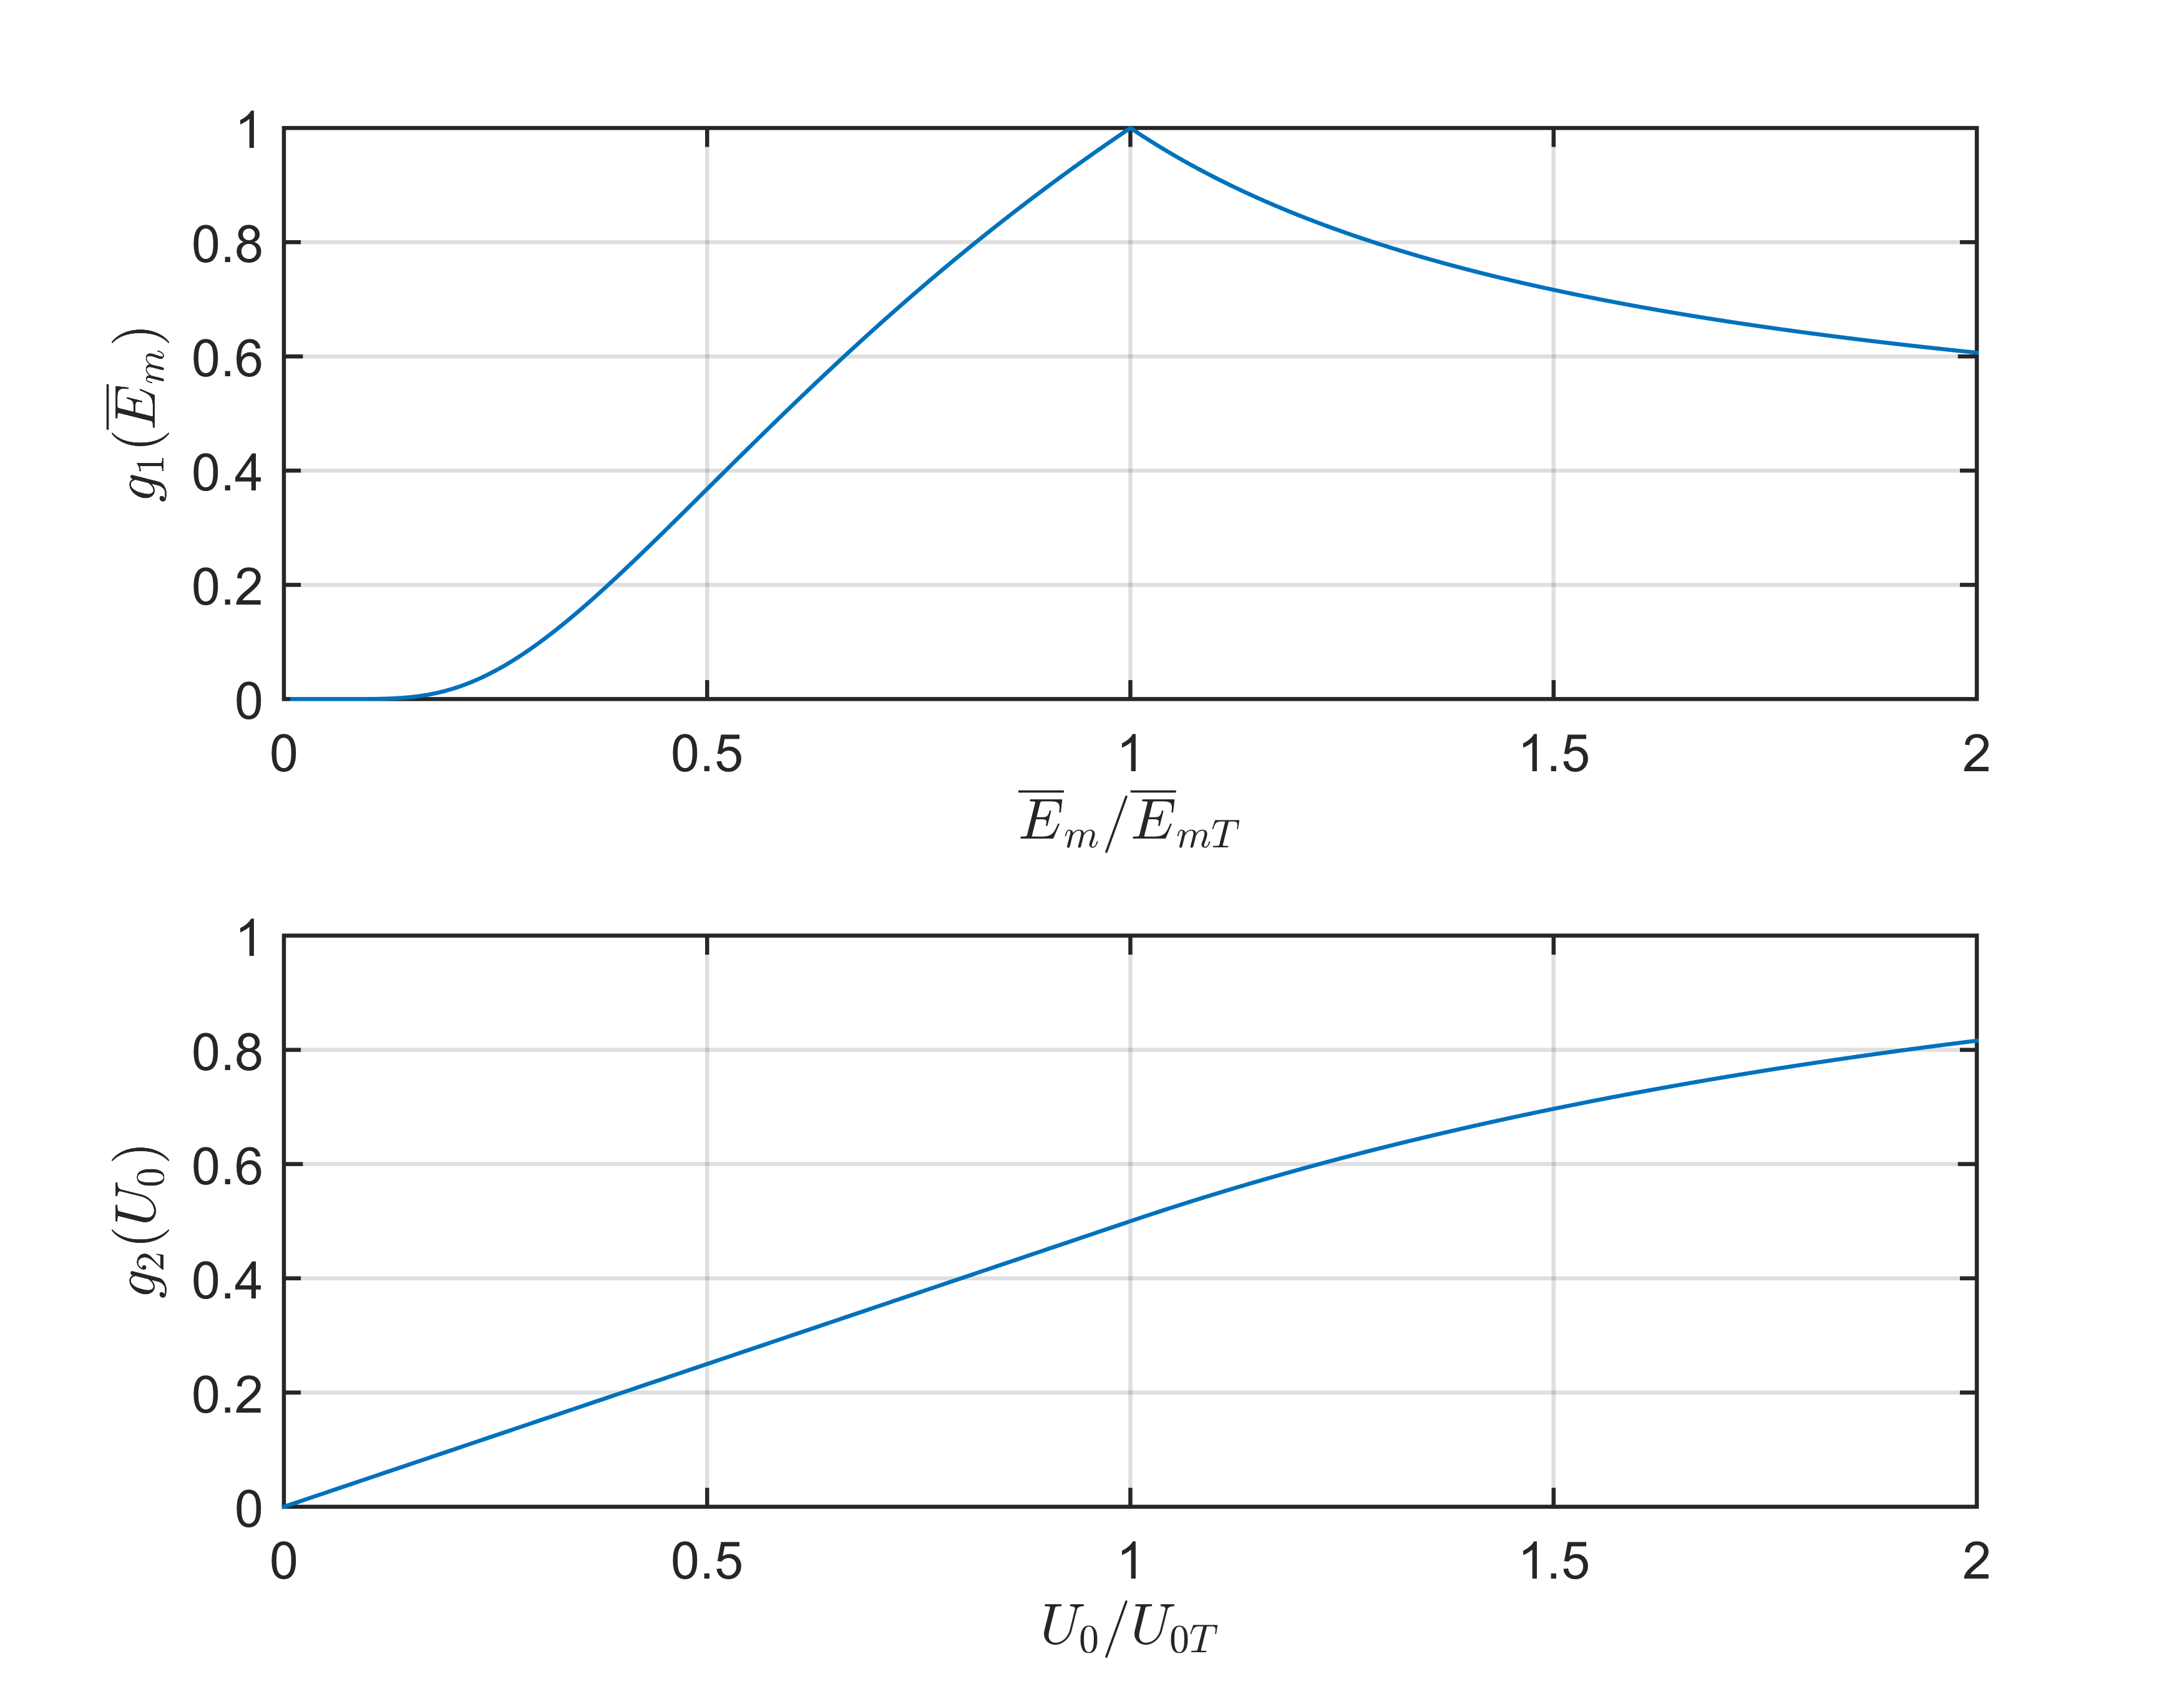
\includegraphics[width=\columnwidth]{obrG1G2}
  \caption{Graphs of parts $g_1\left(\overline{E}_{m}\right)$ and $g_2\left(U_0\right)$ from the fitness function}
  \label{fig:fitG1G2}
\end{figure}

The function $g_2\left(U_{0}\right)$ reach the value $0.5$ at target value of uniformity. It has a bound at $0$ for values less then target value. There is a limit for values in interval higher than target value:
\begin{equation}
\label{eq:g2limInf}
\lim_{U_{0}\to \infty} g_2\left(U_{0}\right) = 1
\end{equation}

So the function $g_2\left(U_{0}\right)$ has an horizontal asymptote equal to one. Function $g_2\left(U_{0}\right)$ is linear for values of uniformity less than the target value. The highest slope is obtained here. For higher values of uniformity is the slope smaller due to the saturation effect of the exponential function. Therefore the algorithm is forced to reach target value of uniformity because of big change in the fitness function. Higher values makes the fitness better too, but there is a smaller effect.
Both functions $g_1\left(\overline{E}_{m}\right)$ and $g_2\left(U_{0}\right)$ are shown in figure~\ref{fig:fitG1G2} for better understanding.
\section{Symmetric Solutions}
One of the requirements to the output design was to get the symmetric solutions of luminaire placement. There seemed to be two approaches how this might be done. The First counts with introduction of the symmetry in the fitness function. On the basis of the fitness equation evaluation the algorithm can prefer symmetric solutions more than others. Unfortunately this approach was very difficult due to unknown function that could describe how good is the symmetry of the luminare placement. Best experience came from using least squares method. After adding the sum of squares of the differences from the average value of ilumminance, a lot of output results showed the symmetry towards axis or center. However some types of luminous intensity distribution curves were very sensitive to create a tight groups of lamps in specific positions. This type of solutions were unable to realize in real conditions.
Authors chose eventually the second approach dealing with introduction of the symmetry in the dna.
\section{Program Behavior}
dva typy symetrie. Pro stredovou jsou vysledky vice kreativni. Pro stredovou symetrii je hladsi prubeh fitness funkce.
Velka souvislost mezi delkou DNA a nastavenou mutaci. Pro velkou mutaci program spatne konverguje. optimalne je pro 200 0.01
Pro nekolik behu vraci program ruzne vysledky, coz v dusledku znamena, ze vice uskupeni splnuje cilove parametry.
Nekdy je vhodne mirne hybat s cilovou hladinou osvetlenosti, jelikoz vzhledem k ostre definici fitness funkce muze dojit k ovlivneni rozmisteni svitidel.
\section{Results in Program Building Design}

% An example of a floating figure using the graphicx package.
% Note that \label must occur AFTER (or within) \caption.
% For figures, \caption should occur after the \includegraphics.
% Note that IEEEtran v1.7 and later has special internal code that
% is designed to preserve the operation of \label within \captio
% even when the captionsoff option is in effect. However, because
% of issues like this, it may be the safest practice to put all your
% \label just after \caption rather than within \caption{}.
%
% Reminder: the "draftcls" or "draftclsnofoot", not "draft", class
% option should be used if it is desired that the figures are to be
% displayed while in draft mode.
%
%\begin{figure}[!t]
%\centering
%\includegraphics[width=2.5in]{myfigure}
% where an .eps filename suffix will be assumed under latex, 
% and a .pdf suffix will be assumed for pdflatex; or what has been declared
% via \DeclareGraphicsExtensions.
%\caption{Simulation Results}
%\label{fig_sim}
%\end{figure}

% Note that IEEE typically puts floats only at the top, even when this
% results in a large percentage of a column being occupied by floats.


% An example of a double column floating figure using two subfigures.
% (The subfig.sty package must be loaded for this to work.)
% The subfigure \label commands are set within each subfloat command, the
% \label for the overall figure must come after \caption.
% \hfil must be used as a separator to get equal spacing.
% The subfigure.sty package works much the same way, except \subfigure is
% used instead of \subfloat.
%
%\begin{figure*}[!t]
%\centerline{\subfloat[Case I]\includegraphics[width=2.5in]{subfigcase1}%
%\label{fig_first_case}}
%\hfil
%\subfloat[Case II]{\includegraphics[width=2.5in]{subfigcase2}%
%\label{fig_second_case}}}
%\caption{Simulation results}
%\label{fig_sim}
%\end{figure*}
%
% Note that often IEEE papers with subfigures do not employ subfigure
% captions (using the optional argument to \subfloat), but instead will
% reference/describe all of them (a), (b), etc., within the main caption.


% An example of a floating table. Note that, for IEEE style tables, the 
% \caption command should come BEFORE the table. Table text will default to
% \footnotesize as IEEE normally uses this smaller font for tables.
% The \label must come after \caption as always.
%
%\begin{table}[!t]
%% increase table row spacing, adjust to taste
%\renewcommand{\arraystretch}{1.3}
% if using array.sty, it might be a good idea to tweak the value of
% \extrarowheight as needed to properly center the text within the cells
%\caption{An Example of a Table}
%\label{table_example}
%\centering
%% Some packages, such as MDW tools, offer better commands for making tables
%% than the plain LaTeX2e tabular which is used here.
%\begin{tabular}{|c||c|}
%\hline
%One & Two\\
%\hline
%Three & Four\\
%\hline
%\end{tabular}
%\end{table}


% Note that IEEE does not put floats in the very first column - or typically
% anywhere on the first page for that matter. Also, in-text middle ("here")
% positioning is not used. Most IEEE journals/conferences use top floats
% exclusively. Note that, LaTeX2e, unlike IEEE journals/conferences, places
% footnotes above bottom floats. This can be corrected via the \fnbelowfloat
% command of the stfloats package.



\section{Conclusion}
Here comes conclusion.



% conference papers do not normally have an appendix



% trigger a \newpage just before the given reference
% number - used to balance the columns on the last page
% adjust value as needed - may need to be readjusted if
% the document is modified later
%\IEEEtriggeratref{8}
% The "triggered" command can be changed if desired:
%\IEEEtriggercmd{\enlargethispage{-5in}}

% references section

% can use a bibliography generated by BibTeX as a .bbl file
% BibTeX documentation can be easily obtained at:
% http://www.ctan.org/tex-archive/biblio/bibtex/contrib/doc/
% The IEEEtran BibTeX style support page is at:
% http://www.michaelshell.org/tex/ieeetran/bibtex/
%\bibliographystyle{IEEEtran}
% argument is your BibTeX string definitions and bibliography database(s)
%\bibliography{IEEEabrv,../bib/paper}
%
% <OR> manually copy in the resultant .bbl file
% set second argument of \begin to the number of references
% (used to reserve space for the reference number labels box)
\begin{thebibliography}{1}
	
\bibitem{CSN_EN_13201-1}
\v{C}SN EN 13201-1. \emph{Road lighting - Part 1: Selection of lighting classes}. march 2007. Prague: \v{C}esk\'{y} normaliza\v{c}n\'{i} institut, 2007.

\bibitem{CSN_EN_13201-2}
\v{C}SN EN 13201-2. \emph{Road lighting - Part 2: Performance requirements}. may 2005. Prague: \v{C}esk\'{y} normaliza\v{c}n\'{i} institut, 2005.

\bibitem{CSN_EN_13201-2_Z1}
\v{C}SN EN 13201-2 ZM\v{E}NA Z1. \emph{Road lighting - Part 2: Performance requirements}. march 2007. Prague: \v{C}esk\'{y} normaliza\v{c}n\'{i} institut, 2007.

\bibitem{CSN_EN_13201-3}
\v{C}SN EN 13201-3. \emph{Road lighting - Part 3: Calculation of performance}. may 2005. Prague: \v{C}esk\'{y} normaliza\v{c}n\'{i} institut, 2005.

\bibitem{Osram}
VIALOX NAV-T SUPER 6Y. OSRAM GMBH. \textit{Osram} [online]. 2015 [cit. 2015-02-18]. Available at: \url{http://www.osram.com/osram_com/products/lamps/high-intensity-discharge-lamps/high-pressure-sodium-vapor-lamps-for-open-and-enclosed-luminaires/vialox-nav-t-super-6y/index.jsp}

\bibitem{Habel}
J. Habel. \textit{Sv\v{e}tlo a osv\v{e}tlov\'{a}n\'{i}}. Praha: FCC Public, 2013, 622~s. ISBN 978-80-86534-21-3.

\bibitem{Zelinka2009}
I. Zelinka, Z. Oplatkov�, M. �eda, P. O�mera, F. V�ela�. \textit{Evolu�n� v�po�etn� techniky: principy a aplikace}. 1. �esk� vyd. Praha: BEN, 2009, 534~s. ISBN 978-80-7300-218-3. 

\bibitem{Fogel2006}
D. B. Fogel. \textit{Evolutionary computation: toward a new philosophy of machine intelligence}. 3rd ed. Hoboken: John Wiley, 2006, xvii, 274~s. ISBN 04-716-6951-2.

\bibitem{Eulumdat}
Eulumdat. \textit{Helios32} [online]. 1999-2014 [cit. 2015-02-19]. Available at: \url{http://www.helios32.com/Eulumdat.htm}

\bibitem{Schreder}
SCHREDER GULF - Products - ATOS. \textit{SCHREDER GULF} [online]. 2015 [cit. 2015-02-19]. Available at: \url{http://www.schreder.com/en-aes/Products/Pages/ATOS.aspx}

\bibitem{CSN EN 12464-1}
\selectlanguage{czech}
\v{C}SN EN 12464-1. \emph{Sv\v{e}tlo a osv\v{e}tlen\'{i} - Osv\v{e}tlen\'{i} pracovn\'{i}ch prostor\r{u}: \v{C}\'{a}st 1: Vnit\v{r}n\'{i} pracovn\'{i} prostory.} Praha: \'{U}\v{r}ad pro technickou normalizaci, metrologii a st\'{a}tn\'{i} zku\v{s}ebnictv\'{i}, 2012
\selectlanguage{english}

\end{thebibliography}



% that's all folks
\end{document}


